% ============================================================================
%  Community Hospital — Presenter Walkthrough & Speaker Script
%  Compile: pdflatex presenter-walkthrough.tex (run twice for TOC)
%  Project slides: ../slides/main.pdf
% ============================================================================
\documentclass[11pt]{article}

\usepackage[utf8]{inputenc}
\usepackage[T1]{fontenc}
\usepackage[a4paper,margin=1in]{geometry}
\usepackage{amsmath,amssymb}
\usepackage{xcolor}
\usepackage[most]{tcolorbox}
\usepackage{enumitem}
\usepackage{booktabs}
\usepackage{array}
\usepackage{graphicx}
\usepackage{fancyhdr}
\usepackage{titlesec}
\usepackage[hidelinks]{hyperref}

\graphicspath{{../slides/figures/}{../slides/}}

% ---- KNUST theme colours ---------------------------------------------------
\definecolor{knustGreen}{HTML}{006B3F}
\definecolor{knustGold}{HTML}{FFD700}
\definecolor{knustDark}{HTML}{1A1A1A}
\definecolor{knustSand}{HTML}{F7F9F8}
\definecolor{knustMuted}{HTML}{4A5568}

\hypersetup{linkcolor=knustGreen, urlcolor=knustGreen}

\titleformat{\section}{\Large\bfseries\color{knustGreen}}{\thesection}{0.6em}{}
\titleformat{\subsection}{\large\bfseries\color{knustDark}}{\thesubsection}{0.6em}{}
\setlist{nosep, leftmargin=1.4em, topsep=2pt}

\newtcolorbox{saybox}{
  enhanced, breakable, colback=knustGreen!6, colframe=knustGreen,
  boxrule=0.8pt, arc=3pt, left=8pt, right=8pt, top=6pt, bottom=6pt,
  fonttitle=\bfseries\color{white}, coltitle=white,
  title={SAY THIS}, attach title to upper={\par\medskip}}

\newtcolorbox{onscreen}{
  enhanced, breakable, colback=knustDark!4, colframe=knustDark!55,
  boxrule=0.6pt, arc=3pt, left=8pt, right=8pt, top=6pt, bottom=6pt,
  fonttitle=\bfseries, coltitle=knustDark,
  title={ON SCREEN}, attach title to upper={\par\smallskip}}

\newtcolorbox{idea}{
  enhanced, breakable, colback=knustGold!12, colframe=knustGold!80!black,
  boxrule=0.6pt, arc=3pt, left=8pt, right=8pt, top=6pt, bottom=6pt,
  fonttitle=\bfseries, coltitle=knustGreen,
  title={THE IDEA}, attach title to upper={\par\smallskip}}

\newtcolorbox{timing}{
  enhanced, colback=knustSand, colframe=knustGold!70!black,
  boxrule=0.5pt, arc=2pt, left=6pt, right=6pt, top=3pt, bottom=3pt,
  fontupper=\small\itshape}

\newtcolorbox{qabox}{
  enhanced, breakable, colback=knustSand, colframe=knustGreen,
  boxrule=0.6pt, arc=3pt, left=8pt, right=8pt, top=6pt, bottom=6pt,
  fonttitle=\bfseries, coltitle=knustGreen,
  title={LIKELY QUESTION \& ANSWER}, attach title to upper={\par\smallskip}}

\newcommand{\transition}[1]{\medskip\noindent\textit{\textcolor{knustMuted}{Transition: #1}}\medskip}
\newcommand{\deck}[1]{{\small\texttt{\textcolor{knustMuted}{main.pdf slide: #1}}}}

\newcommand{\slide}[3]{%
  \subsection{Slide #1 --- #2}%
  \noindent\deck{#1 --- #3}\par\smallskip}

\pagestyle{fancy}
\fancyhf{}
\fancyhead[L]{\small\textcolor{knustGreen}{Hospital Chatbot --- Presenter Walkthrough}}
\fancyhead[R]{\small\textcolor{knustMuted}{KNUST FYP 2026}}
\fancyfoot[C]{\small\thepage}
\renewcommand{\headrulewidth}{0.4pt}

% ============================================================================
\begin{document}

\begin{titlepage}
\centering
\vspace*{2.5cm}
{\Huge\bfseries\color{knustGreen} Hospital Chatbot}\\[0.3cm]
{\LARGE\bfseries for Color Coded Clinical Pathways}\\[1cm]
{\Large\itshape Presenter Walkthrough \& Speaker Script}\\[0.5cm]
{\large Step-by-step guide for all 20 slides in \texttt{main.pdf}}\\[2cm]
{\large Quaigraine Samuel \\ Twum Samuel}\\[0.3cm]
{\large Department of Mathematics, KNUST}\\[0.3cm]
{\large August 2026}\\[1.5cm]
\begin{tcolorbox}[width=0.88\textwidth, colback=knustSand, colframe=knustGreen, arc=4pt]
\small\centering
Project \textbf{main.pdf} on the projector; keep \textbf{this handbook} on your laptop or print it.
Each section matches one Beamer slide in order. Read the \textbf{SAY THIS} boxes aloud or paraphrase.
\end{tcolorbox}
\end{titlepage}

\tableofcontents
\newpage

% ============================================================================
\section{How to use this handbook}

\begin{itemize}
  \item \textbf{Structure.} Twenty slides in \texttt{community-hospital/slides/main.pdf}, in fixed order.
        This document has one subsection per slide.
  \item \textbf{Coloured boxes.}
    \begin{itemize}
      \item \textbf{ON SCREEN} --- what the audience sees; point at it while speaking.
      \item \textbf{THE IDEA} --- plain-language concept (math/OR slides).
      \item \textbf{SAY THIS} --- full spoken script with verbal citations.
    \end{itemize}
  \item \textbf{Citations.} Slides show author--year in parentheses; name them aloud
        (e.g.\ ``Mitchell and colleagues, twenty twenty-three'').
  \item \textbf{Our numbers.} Say ``in our Community Hospital case study'' for metrics tagged This study, 2026.
\end{itemize}

\subsection*{Pre-flight checklist}
\begin{enumerate}
  \item Open \texttt{main.pdf} full-screen on the projector.
  \item Have this PDF on a second screen or printed.
  \item Confirm chart images render (slides 7--10, 15).
  \item Optional: open \texttt{community\_hospital\_patients.csv} if asked about data.
\end{enumerate}

\subsection*{Timing overview}
\begin{center}
\small
\begin{tabular}{@{}clcc@{}}
\toprule
Slides & Section & Slides & Minutes \\
\midrule
1--2 & Opening & 2 & 2 \\
3--4 & Research gaps & 2 & 4 \\
5--11 & Community Hospital case study & 7 & 10 \\
12--15 & Transshipment optimization & 4 & 6 \\
16--17 & NLP triage design & 2 & 4 \\
18--20 & Conclusion \& references & 3 & 4 \\
\midrule
& \textbf{Total} & \textbf{20} & \textbf{25--30} \\
\bottomrule
\end{tabular}
\end{center}

\subsection*{Key numbers cheat sheet}
\begin{itemize}[noitemsep]
  \item $N = 1000$; skewed mix 5\% / 15\% / 30\% / 25\% / 25\%
  \item Colour-routing accuracy: \textbf{97.5\%} (975/1000)
  \item Level 1 recall: \textbf{94.0\%} (47/50)
  \item Green diversion: \textbf{500} patients (50\%)
  \item Transshipment: cost 7150 $\to$ 2700 (\textbf{62\%}); acute load 900 $\to$ 500 (\textbf{44\%})
  \item 8k BioBERT holdout reference: 99.92\%
\end{itemize}

\newpage
\section{Slide-by-slide walkthrough}

% --- SLIDE 1 ----------------------------------------------------------------
\slide{1}{Title}{Opening}
\begin{timing}Suggested: 30 sec\end{timing}
\begin{onscreen}
Title: \emph{Hospital Chatbot for Color Coded Clinical Pathways}. Subtitle: Community Hospital case study.
Authors: Quaigraine Samuel, Twum Samuel. KNUST Mathematics, August 2026.
\end{onscreen}
\begin{saybox}
Good morning everyone. Thank you for being here. Today we present our final-year project:
\textbf{Hospital Chatbot for Color Coded Clinical Pathways}. We use a synthetic Community Hospital
case study in Ghana to show how free-text chief complaints can map to SATS colours and pathway cards,
and how that can reduce emergency-department overcrowding. I am Quaigraine Samuel, and my colleague
is Twum Samuel, from the Department of Mathematics at KNUST.
\end{saybox}
\transition{Advance to the outline.}

% --- SLIDE 2 ----------------------------------------------------------------
\slide{2}{Outline of Presentation}{Opening}
\begin{timing}Suggested: 1 min\end{timing}
\begin{onscreen}
Table of contents: Research gaps; Community Hospital case study; Transshipment optimization;
NLP triage design; Conclusion; References.
\end{onscreen}
\begin{saybox}
Here is the road map. We start with \textbf{research gaps} in prior work---why text-based pre-triage
matters for overcrowding. Then our \textbf{Community Hospital} synthetic evaluation with a thousand
skewed cases. Next, \textbf{transshipment optimization} models patient flow as a network problem.
We explain \textbf{NLP design}---conversational intake but constrained outputs, not a generic chatbot.
We close with \textbf{summary, limitations}, and full \textbf{references}.
\end{saybox}
\transition{Open with real-world ED overcrowding images.}

% --- SLIDE 3 ----------------------------------------------------------------
\slide{3}{ED overcrowding and waiting for care}{Research gaps}
\begin{timing}Suggested: 2 min\end{timing}
\begin{onscreen}
Two photos side by side with source lines:
\begin{itemize}[noitemsep]
  \item Left: Longdon (2026), Citi Newsroom --- queue for care.
  \item Right: Aminu (2021), Ghana Fact --- Korle-Bu overcrowding fact-check.
\end{itemize}
\end{onscreen}
\begin{center}
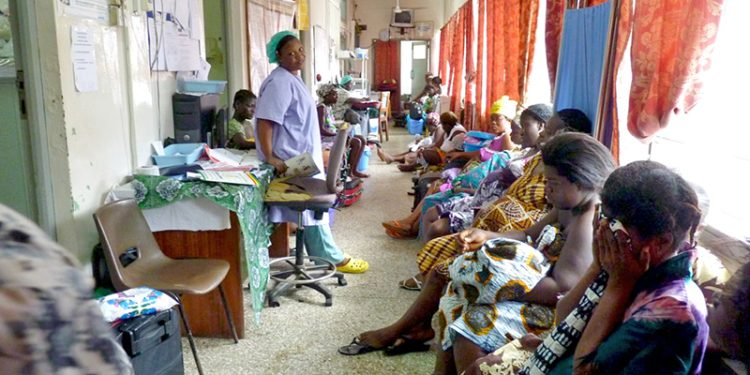
\includegraphics[width=0.42\textwidth]{image1.jpg}\hfill
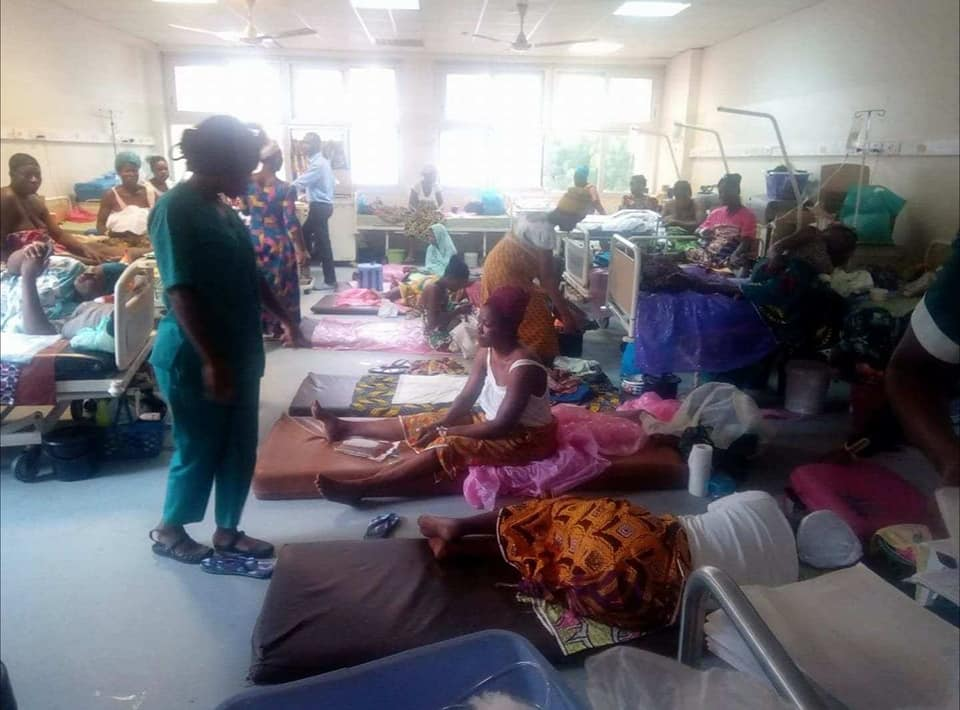
\includegraphics[width=0.42\textwidth]{image2.jpg}
\end{center}
\begin{saybox}
Before the literature, look at the reality. On the left, Bervelyn Longdon's twenty twenty-six
Citi Newsroom piece on \emph{queue for care}---patients waiting because the system is stretched.
On the right, Ghana Fact's twenty twenty-one fact-check on Korle-Bu Teaching Hospital overcrowding:
hallways and wards under pressure. These are not abstract statistics; they are why we care about
\textbf{routing the right patient to the right queue early}. Our project asks: can we estimate urgency
from words \emph{before} vitals and the physical triage desk, to reduce this congestion?
\end{saybox}
\transition{State the five literature gaps on one slide.}

% --- SLIDE 4 ----------------------------------------------------------------
\slide{4}{Research gaps in prior work}{Research gaps}
\begin{timing}Suggested: 2--3 min\end{timing}
\begin{onscreen}
Intro sentence plus five numbered one-line gaps, each with author--year citations
(SATS 2012; Rominski et al.\ 2014; Stewart et al.\ 2023; Mitchell et al.\ 2023; Yilmaz 2021; etc.).
\end{onscreen}
\begin{saybox}
Our aim is to infer acuity from free-form chief complaints to reduce ED overcrowding and waiting times---
Mitchell and colleagues in twenty twenty-three and Yilmaz in twenty twenty-one frame that problem.

\textbf{Gap one, vitals-first bias:} SATS and TEWS assume bedside physiology first; Stewart's twenty
twenty-three NLP review shows few systems estimate acuity from text when vitals are still unknown.

\textbf{Gap two, pathway discontinuity:} colours are assigned at the desk, but Nurchis et al.\ twenty
twenty-five and Sundstr\"om et al.\ twenty fourteen show waiting-time and destination protocols are
not always carried forward digitally.

\textbf{Gap three, overcrowding without text pre-triage:} Green-tag patients congest acute zones---
Yilmaz and Mitchell again.

\textbf{Gap four, generative versus constrained NLP:} open-ended chatbots raise hallucination risk;
Stewart and Cheng et al.\ twenty twenty-five contrast that with fixed acuity classes.

\textbf{Gap five, class imbalance:} papers report overall accuracy but under-report recall on rare
Red cases---Stewart and Berkowitz et al.\ on under-triage safety.

These are gaps in \emph{prior work}; our case study addresses them next.
\end{saybox}
\transition{Introduce the Community Hospital synthetic cohort.}

% --- SLIDE 5 ----------------------------------------------------------------
\slide{5}{Case study setting}{Community Hospital}
\begin{timing}Suggested: 2 min\end{timing}
\begin{onscreen}
Bullets: fictional Kumasi-region LMIC hospital; $N=1000$ skewed mix; Ghanaian complaints; SATS labels
and pathways; 7\% ambiguity flag; 97.5\% colour accuracy; 99.92\% holdout reference.
\end{onscreen}
\begin{saybox}
We built a \textbf{Community Hospital}---a fictional but Kumasi-region-style LMIC facility, grounded in
Rominski's KATH SATS work and Gyedu on trainee triage in Ghana. We generated \textbf{one thousand}
synthetic patients with a \textbf{realistic skewed mix}: five, fifteen, thirty, twenty-five, twenty-five
percent across acuity levels---not a balanced toy dataset, following Mitchell on LMIC ED statistics.

Each row has Ghanaian patient-voice complaints---Kejetia, Bantama, Ejisu, Sunyani, KATH references.
Nurse ground truth maps level to SATS colour and pathway card. About \textbf{seven percent} are flagged
borderline. In our case study the chatbot achieves \textbf{ninety-seven point five percent}
colour-routing accuracy; separately, BioBERT on an eight-thousand holdout reaches ninety-nine point
ninety-two percent---Lee et al.\ twenty twenty on BioBERT.
\end{saybox}
\transition{Show the CSV schema briefly.}

% --- SLIDE 6 ----------------------------------------------------------------
\slide{6}{Dataset schema}{Community Hospital}
\begin{timing}Suggested: 1 min\end{timing}
\begin{onscreen}
Table: patient\_id, demographics, chief\_complaint, acuity\_level, sats\_colour, pathway\_destination,
t\_max\_minutes, ambiguity\_flag. Path to CSV file.
\end{onscreen}
\begin{saybox}
This slide is for transparency. Every synthetic patient row carries an ID, demographics, the full
chief complaint text, nurse acuity level one to five, SATS colour, \textbf{pathway destination},
\textbf{time target} in minutes, and an ambiguity flag. The file lives at
\texttt{community-hospital/data/community\_hospital\_patients.csv}. The point is: we do not only predict
a colour---each row binds colour to operational routing data.
\end{saybox}
\transition{Show the acuity bar chart.}

% --- SLIDE 7 ----------------------------------------------------------------
\slide{7}{Acuity distribution}{Community Hospital}
\begin{timing}Suggested: 1--2 min\end{timing}
\begin{onscreen}
Bar chart \texttt{acuity\_distribution.png}. Caption: skewed mix; L4/L5 distinct shades, both Green.
\end{onscreen}
\begin{center}
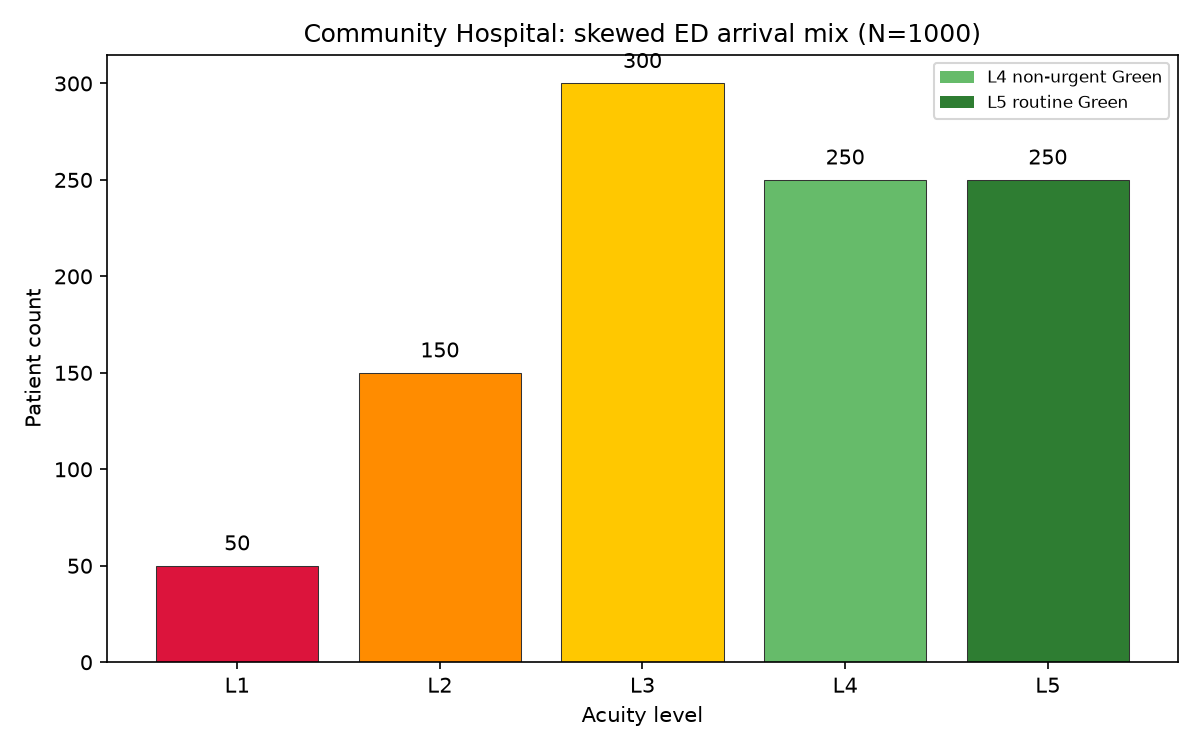
\includegraphics[width=0.72\textwidth]{acuity_distribution.png}
\end{center}
\begin{saybox}
This chart shows our \textbf{skewed arrival mix}---few critical Reds, many Yellows and Greens, as in
real EDs per Mitchell and Rominski. Notice levels four and five use \textbf{different bar colours} but
both map to SATS Green---that matters when we discuss accuracy by level later.
\end{saybox}
\transition{Show pathway flow chart.}

% --- SLIDE 8 ----------------------------------------------------------------
\slide{8}{Pathway destinations}{Community Hospital}
\begin{timing}Suggested: 1--2 min\end{timing}
\begin{onscreen}
Chart \texttt{pathway\_flow.png}. Plain block: every row has destination and $T_{\max}$; colour binds to protocol.
\end{onscreen}
\begin{center}
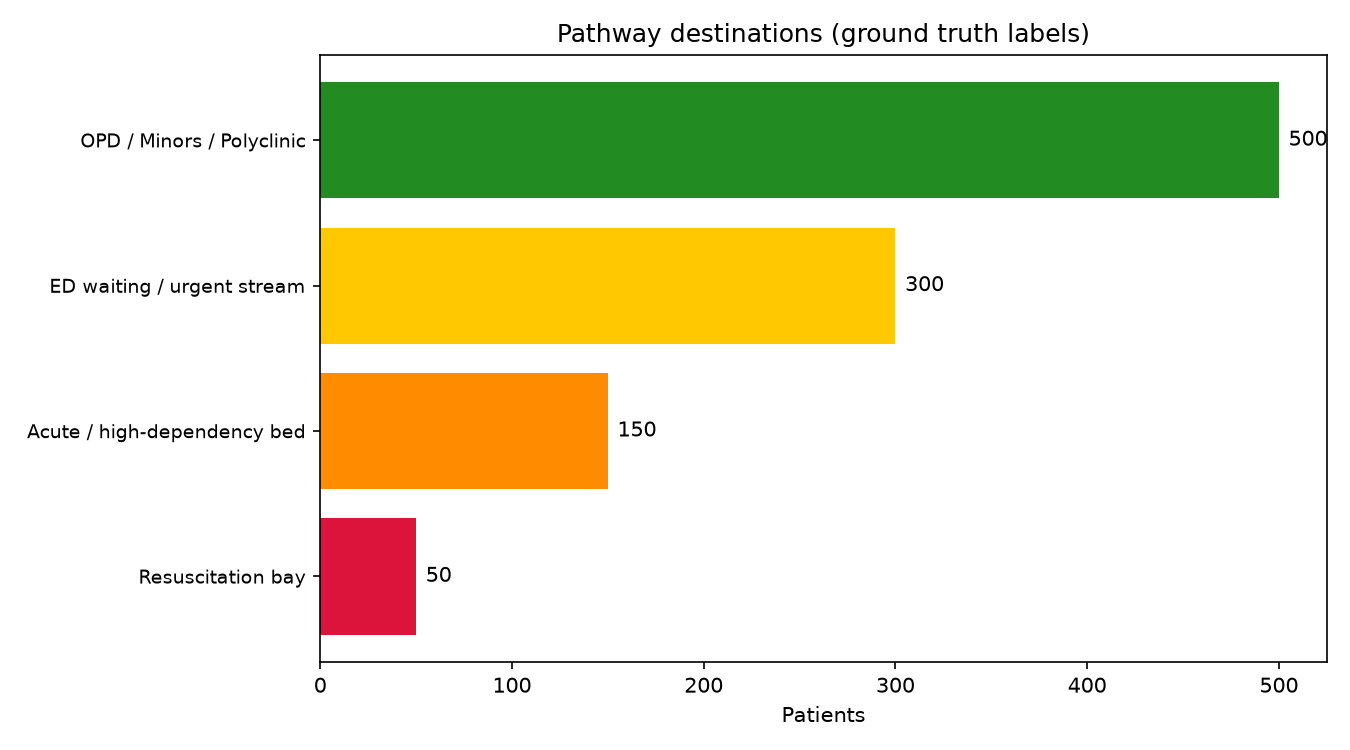
\includegraphics[width=0.72\textwidth]{pathway_flow.png}
\end{center}
\begin{saybox}
Colour is not a sticker---it must mean a \textbf{protocol}. Sundstr\"om et al.\ on pathway care and the
SATS manual show destination and time target matter. Here, Orange routes to acute beds within ten
minutes; Green to OPD or minors within hours. Every CSV row carries that pathway card, not just a label.
\end{saybox}
\transition{Discuss Green diversion and overcrowding.}

% --- SLIDE 9 ----------------------------------------------------------------
\slide{9}{Green-pathway diversion}{Community Hospital}
\begin{timing}Suggested: 2 min\end{timing}
\begin{onscreen}
Left: \texttt{green\_diversion.png}. Right: 50\% of cohort ($n=500$) to OPD/Minors; chatbot assigns Green at intake.
\end{onscreen}
\begin{center}
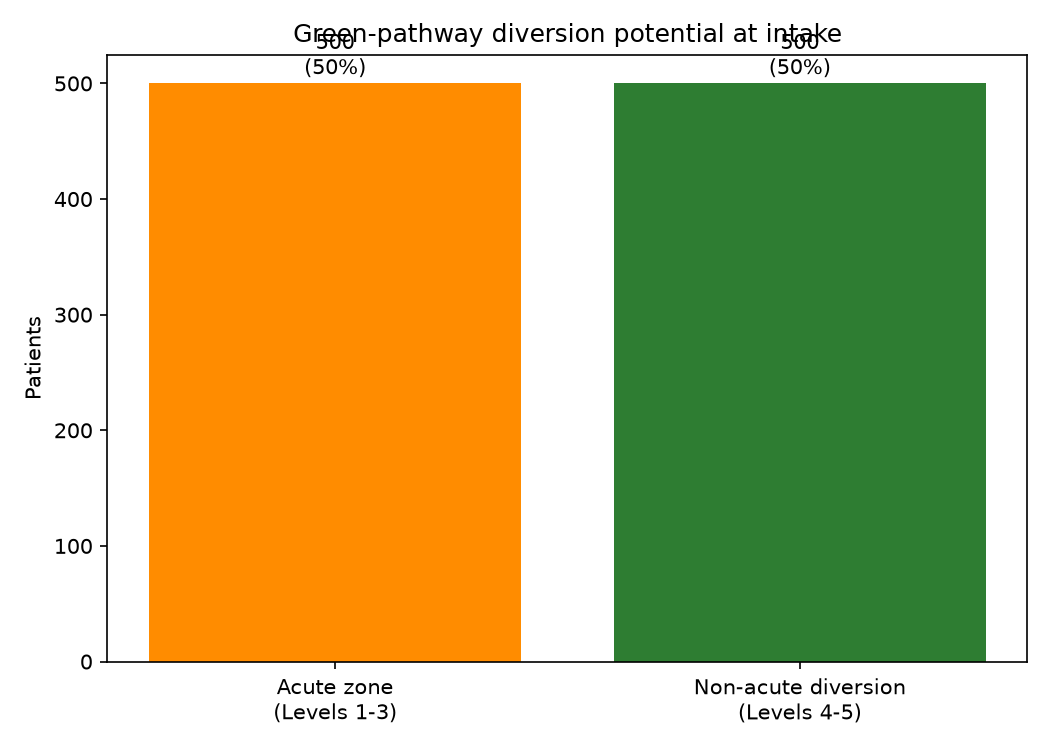
\includegraphics[width=0.55\textwidth]{green_diversion.png}
\end{center}
\begin{saybox}
Half our cohort---five hundred patients at levels four and five---are \textbf{Green diversion candidates}
routed to OPD, Minors, or Polyclinic in our case study. Yilmaz's Green-tag burden and Mitchell's
overcrowding work explain why that matters: without early diversion, non-urgent patients queue in
acute zones. Our chatbot assigns Green \textbf{at intake}, before the physical desk---Sundstr\"om-style
pathway routing applied early.
\end{saybox}
\transition{Show per-level accuracy chart.}

% --- SLIDE 10 ---------------------------------------------------------------
\slide{10}{Chatbot colour-routing accuracy}{Community Hospital}
\begin{timing}Suggested: 2 min\end{timing}
\begin{onscreen}
Chart \texttt{chatbot\_accuracy\_by\_level.png}. 97.5\% overall; L1 recall 94\% (47/50).
\end{onscreen}
\begin{center}
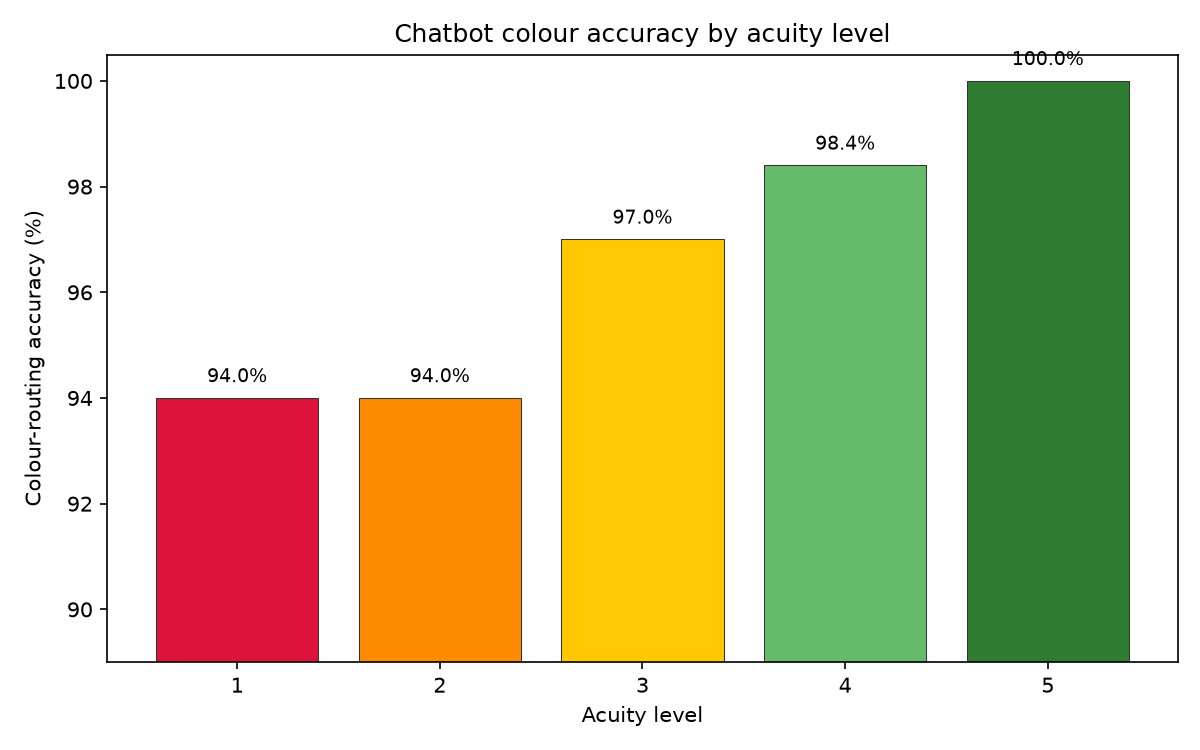
\includegraphics[width=0.72\textwidth]{chatbot_accuracy_by_level.png}
\end{center}
\begin{saybox}
Overall \textbf{ninety-seven point five percent} colour-routing---nine hundred seventy-five of one thousand.
Level-one recall is \textbf{ninety-four percent}---forty-seven of fifty Reds---the safety-critical minority
under skewed priors, as Stewart and Berkowitz warn. Errors cluster on \textbf{adjacent levels} and the
seven percent borderline flag rows. We report per-level metrics, not accuracy alone.
\end{saybox}
\transition{Summarise case study findings.}

% --- SLIDE 11 ---------------------------------------------------------------
\slide{11}{Case study conclusion}{Community Hospital}
\begin{timing}Suggested: 1--2 min\end{timing}
\begin{onscreen}
Findings block: NLP to SATS before vitals; pathway on every row; 500 Green diversion lever. Plain: next transshipment LP.
\end{onscreen}
\begin{saybox}
Three takeaways from the case study. First, NLP maps Ghanaian free text to SATS colour \textbf{before
vitals}---Stewart and Gligorijevi\'c on text triage, confirmed in our cohort. Second, every case includes
destination and $T_{\max}$---pathway continuity. Third, five hundred Green diversions are an operational
lever on crowding per Yilmaz. Next we model ED flow as a \textbf{transshipment network}.
\end{saybox}
\transition{Introduce the LP framing.}

% --- SLIDE 12 ---------------------------------------------------------------
\slide{12}{ED overcrowding as a network problem}{Transshipment}
\begin{timing}Suggested: 1--2 min\end{timing}
\begin{onscreen}
Problem statement; transshipment LP $\min Z = \sum c_{ij} x_{ij}$; supply/balance/demand; plain block on flow metaphor.
\end{onscreen}
\begin{idea}
Think of patients as \textbf{flow} and hospital zones as \textbf{nodes}. A transshipment LP minimises
total routing cost: expected wait plus penalty for wrong-queue assignment. The chatbot is a cheap
transshipment node that diverts Green patients before they hit majors.
\end{idea}
\begin{saybox}
Overcrowding is not only a queue length statistic---Yilmaz and Mitchell---it is a \textbf{routing} problem.
When non-urgent patients enter the acute queue, everyone waits longer. We model this as a
transshipment linear program: minimise total cost $Z$ over arcs $x_{ij}$, subject to supply at arrival
streams, balance at intermediate nodes, and demand at resuscitation, majors, and OPD. In our Community
Hospital instance, cost combines wait and wrong-queue penalty.
\end{saybox}
\transition{Walk through the network diagram.}

% --- SLIDE 13 ---------------------------------------------------------------
\slide{13}{Hospital transshipment network}{Transshipment}
\begin{timing}Suggested: 2 min\end{timing}
\begin{onscreen}
TikZ diagram: three layers (Sources, Transshipment, Destinations). Arrivals (50, 150, 300, 500) $\to$
chatbot + desk $\to$ resus, majors, OPD.
\end{onscreen}
\begin{saybox}
Top row: four arrival \textbf{sources}---Critical fifty, Very urgent one fifty, Urgent three hundred,
Non-urgent five hundred---matching our skewed cohort totals. Middle row: \textbf{transshipment nodes}---
chatbot pre-triage and the physical triage desk. Bottom row: \textbf{destinations}---resuscitation fifty,
majors four fifty, OPD five hundred. Trace arcs: most non-urgent flow can pass through the chatbot early;
urgent three hundreds may still hit the desk. Point to layer labels on the left so the audience reads
top-down.
\end{saybox}
\transition{Show the LP table with numbers.}

% --- SLIDE 14 ---------------------------------------------------------------
\slide{14}{LP structure}{Transshipment}
\begin{timing}Suggested: 2 min\end{timing}
\begin{onscreen}
Decision variables $x_{ij}$; supply/demand numbers; block table: without chatbot $Z=7150$, acute load 900;
with chatbot $Z=2700$, load 500; 62\% and 44\% reductions.
\end{onscreen}
\begin{saybox}
Decision variables $x_{ij}$ count patients on each arc. Supplies match arrivals; demands match bed
targets. \textbf{Without} digital pre-triage, total cost is seven thousand one hundred fifty and
\textbf{nine hundred} patients load the acute zone---Green mis-routes to majors. \textbf{With} the
chatbot transshipment node, cost drops to two thousand seven hundred---a \textbf{sixty-two percent}
reduction---and acute load falls to five hundred---\textbf{forty-four percent}. These are analytical
results from our Community Hospital case study, not a deployed hospital optimizer yet.
\end{saybox}
\transition{Show the scenario chart.}

% --- SLIDE 15 ---------------------------------------------------------------
\slide{15}{Acute-zone load reduction}{Transshipment}
\begin{timing}Suggested: 1--2 min\end{timing}
\begin{onscreen}
Chart \texttt{wait\_time\_scenario.png}. Plain: 500 Green patients can mis-route without pre-triage.
\end{onscreen}
\begin{center}
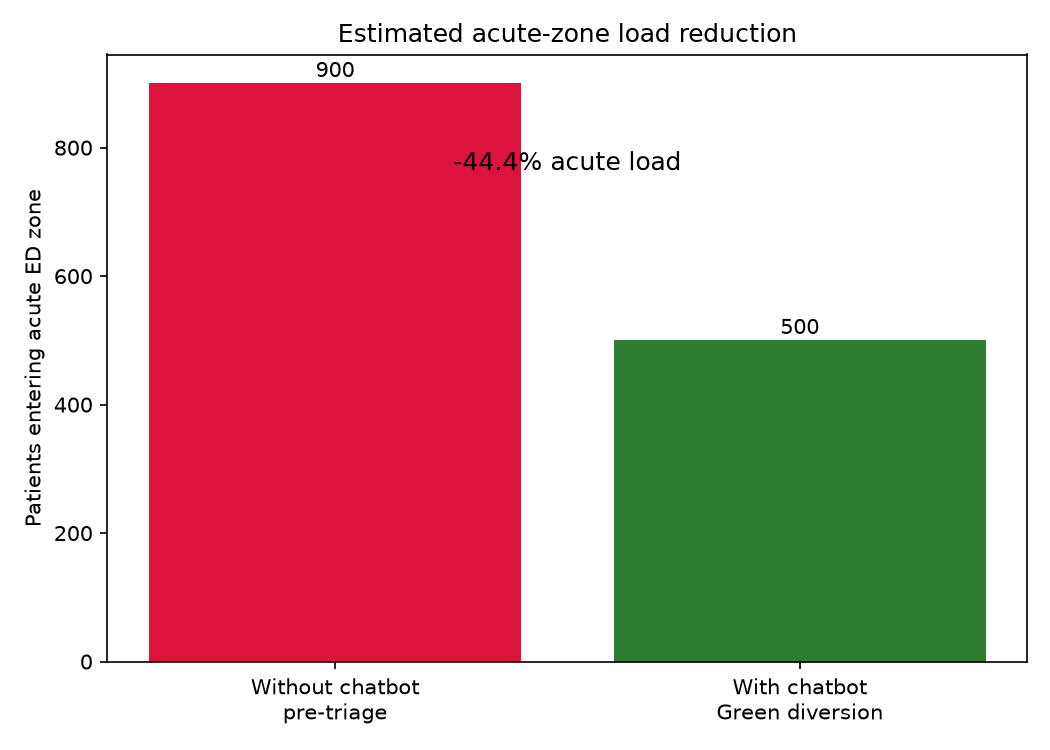
\includegraphics[width=0.72\textwidth]{wait_time_scenario.png}
\end{center}
\begin{saybox}
This chart visualises the scenario comparison. Without early Green diversion---Yilmaz's overcrowding
picture---five hundred low-acuity patients can inflate majors queues. With chatbot pre-triage they shift
to OPD early in our model. The OR story supports the clinical story: text-based acuity is not only
classification; it is a \textbf{flow-management} lever.
\end{saybox}
\transition{Switch to NLP system design.}

% --- SLIDE 16 ---------------------------------------------------------------
\slide{16}{Conversational NLP supports triage}{NLP design}
\begin{timing}Suggested: 2 min\end{timing}
\begin{onscreen}
Bullets on chat intake, optional voice/OpenMed; fixed outputs block: $\hat{c}$, $C=f_{\mathrm{SATS}}(\hat{c})$, $P(C)$.
\end{onscreen}
\begin{saybox}
The chatbot is \textbf{conversational}---patients speak in Ghanaian English with local context---Stewart
and An et al.\ on conversational health agents. Optional voice, medical gate, OpenMed tags sit on
BioBERT per Lee et al. But output is \textbf{not} free-form medical advice---Cheng on triage under
uncertainty. Fixed outputs only: predicted acuity one to five; SATS colour via deterministic map;
pathway card with destination, $T_{\max}$, actions---Sundstr\"om and SATS protocol.
\end{saybox}
\transition{Contrast with generative LLMs.}

% --- SLIDE 17 ---------------------------------------------------------------
\slide{17}{Versus generative clinical chatbots}{NLP design}
\begin{timing}Suggested: 2 min\end{timing}
\begin{onscreen}
Two-column table: Generative LLM vs Curatio---open text vs fixed class; hallucination vs bounded set; audit vs metrics.
Plain: nurse remains in the loop.
\end{onscreen}
\begin{saybox}
Why not ChatGPT? Generative models give open-ended replies---An et al.---with hallucination risk Stewart
flags. We output a \textbf{bounded set}: class, colour, pathway card---auditable with confidence and
per-level metrics in our case study. Instead of ``you might have pneumonia,'' we say ``Orange, acute bed,
ten minutes'' per SATS. The nurse remains in the loop---Cheng and Rominski---pre-triage and route, not
replace clinical judgment.
\end{saybox}
\transition{Close with summary.}

% --- SLIDE 18 ---------------------------------------------------------------
\slide{18}{Summary}{Conclusion}
\begin{timing}Suggested: 2 min\end{timing}
\begin{onscreen}
Four numbered takeaways: gaps; case study numbers; transshipment reductions; NLP design.
\end{onscreen}
\begin{saybox}
Four closing points. \textbf{One:} prior gaps---text before vitals, pathway continuity, overcrowding,
constrained NLP, class imbalance---Stewart, Sundstr\"om, Mitchell. \textbf{Two:} Community Hospital---
one thousand skewed cases, ninety-seven point five percent accuracy, pathway on every row. \textbf{Three:}
transshipment OR---sixty-two percent cost and forty-four percent acute-load reduction with Green
diversion. \textbf{Four:} NLP design---conversation in, fixed acuity and pathway out, not generative
diagnosis---Lee and Cheng.
\end{saybox}
\transition{Acknowledge limitations honestly.}

% --- SLIDE 19 ---------------------------------------------------------------
\slide{19}{Limitations}{Conclusion}
\begin{timing}Suggested: 1--2 min\end{timing}
\begin{onscreen}
Three bullets: synthetic cohort; simulated eval / holdout reference; analytical transshipment only.
\end{onscreen}
\begin{saybox}
We are transparent on limits. \textbf{First}, synthetic cohort---not yet prospective validation at KATH
where Rominski validated SATS. \textbf{Second}, case-study chatbot eval was simulated when the ML
service was offline; BioBERT holdout at ninety-nine point ninety-two percent is the separate reference.
\textbf{Third}, transshipment is an analytical model---Mitchell's LMIC triage impact work sets context---not
a deployed hospital optimizer today.
\end{saybox}
\transition{End on references; invite questions.}

% --- SLIDE 20 ---------------------------------------------------------------
\slide{20}{References}{Closing}
\begin{timing}Suggested: 1 min (do not read every line)\end{timing}
\begin{onscreen}
Full bibliography from \texttt{references.bib} (allow frame breaks).
\end{onscreen}
\begin{saybox}
Full references are on screen---SATS manual, Rominski, Stewart, Mitchell, Yilmaz, Lee on BioBERT, and
our This study twenty twenty-six case-study entry. I will not read every line aloud; the PDF and
\texttt{references.bib} are available. Thank you---we welcome your questions.
\end{saybox}

\newpage
% ============================================================================
\section{Anticipated Q\&A}

\begin{qabox}
\textbf{Q: Why synthetic data?}\\
\textbf{A:} Real ED data is hard to release; we need a skewed mix---five-fifteen-thirty-twenty-five-twenty-five---
to mirror Mitchell on LMIC statistics. BioBERT is validated separately on an eight-thousand holdout at
ninety-nine point ninety-two percent.
\end{qabox}

\begin{qabox}
\textbf{Q: Why not ChatGPT?}\\
\textbf{A:} Bounded acuity class and pathway card; no hallucinated urgency. Stewart's review and our
comparison table on slide seventeen---fixed outputs, per-level metrics, nurse in the loop.
\end{qabox}

\begin{qabox}
\textbf{Q: Why two greens on the chart?}\\
\textbf{A:} Levels four and five are different acuity levels---non-urgent versus routine---but both map
to SATS Green per the manual. Distinct bar colours on slide seven; same routing colour.
\end{qabox}

\begin{qabox}
\textbf{Q: Is TEWS included?}\\
\textbf{A:} Not in this case-study chatbot path---vitals-first gap from slide four. TEWS remains nurse-side;
future fusion is documented in \texttt{triage-fusion/} at repo root.
\end{qabox}

\section{Rebuild commands}

\begin{verbatim}
cp community-hospital/analysis/figures/*.png community-hospital/slides/figures/
cd community-hospital/slides
pdflatex main.tex && bibtex main && pdflatex main.tex && pdflatex main.tex
cd ../guide
pdflatex presenter-walkthrough.tex && pdflatex presenter-walkthrough.tex
\end{verbatim}

\end{document}
